\documentclass[journal, a4paper]{IEEEtran}
\usepackage{graphicx}   
\usepackage[utf8]{inputenc}
\usepackage{natbib}
\usepackage{url}     
\usepackage{amsmath}    
\usepackage{float}
\begin{document}

% Define document title and author 
	\title{Energy Harvesting y Energy Scavenging}
	\author{Saul Luna Minor 201443135
	\\Facultad de Ciencias de la Electrónica, BUAP. Av. San Claudio y 18 sur. Puebla - MÉXICO
	\\ctiocalvis@gmail.com}
	\markboth{Sistemas de generación y optimización de Energía 1. 9, Enero 2019}{}
	\maketitle

% Write abstract here
\begin{abstract}
  El trabajo presente es una investigación sobre Energy Harvesting y Energy Scavenging, donde se compara ambos conceptos, así como se describen algunos ejemplos. Al final se da una conclusión de la relevancia que tienen los términos actualmente.  
\end{abstract}

% Each section begins with a \section{title} command
\section{Introducción}
	Los conceptos son bastante semejantes, sin embargo, estos se diferencian entre si. Energy Scavenging\citep{Priya2009} se refiere a entornos donde las fuentes ambientales son desconocidas o muy irregulares mientras que Enegy Harvesting\citep{Priya2009}  recolecta energía de fuentes bien caracterizadas y más regulares. Más adelante se abordara ejemplos de cada uno de los conceptos. 

% Main Part
\section{Discusión Energy Scavenging y Energy Harvesting}
Hay controversia de que se considera que es Energy Harvesting o Scavenging, por ejemplo cuando se habla de energía solar, el sol como tal no esta caracterizado, por lo cual se podría considerar Energy Scavenging, sin embargo, si se habla de fotones de luz, que irradia el sol, entonces se tiene una partícula caracterizada por lo cual se habla de Energy Harvesting. En la literatura, en ocasiones ambos conceptos son empleados con el mismo significado, por lo que no se difiere uno del otro. 

\section{Nuevas tecnologías}
\subsection{Electronic-skin\citep{Nunez2019} (piel eléctrica)}
Este concepto abarca las investigaciones sobre implantar ó poner sobre la piel sensores microscópicos, que permitan medir varios parámetros como son: latidos, presión, temperatura del cuerpo. Estos sensores requieren baterías que llegan a ser estorbosas, por lo que se opto el uso de polímeros\citep{Nunez2019} piezoeléctricos(Figura 1), los cuales obtienen energía cuando se les deforman. 


\begin{figure}[H]
\centering
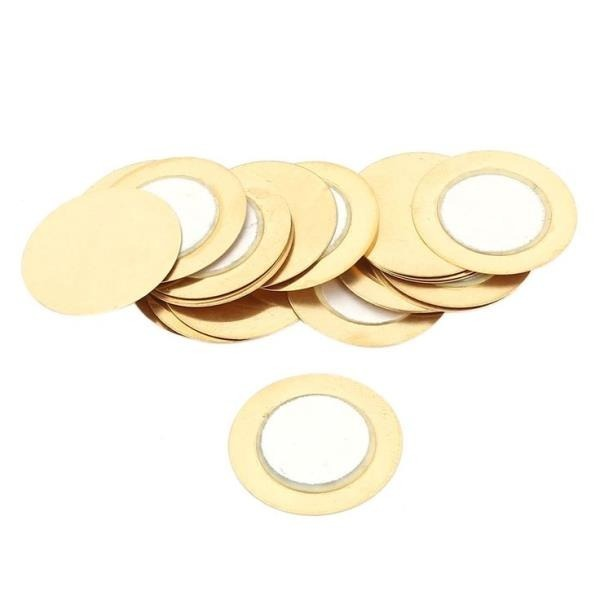
\includegraphics[scale=0.2]{figura1.jpg}
\caption{Material piezoeléctrico más común.}
\label{fig:figura1}
\end{figure}
\subsection{Baterías a micro-escala\citep{Roundy2005}}
Estas baterías están diseñadas para almacenar hasta 4.2V, con el inconveniente de tener una corriente máxima de 5mA, con lo cual puede llegar a prender un diodo led, que consuma esa corriente. Estas son ideales por su pequeño tamaño.Se obtienen de una oblea de silicio(Figura 2). 
\begin{figure}[H]
\centering
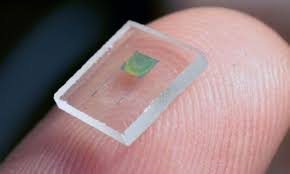
\includegraphics[scale=0.5]{ubateria.jpg}
\caption{Comparativa de tamaño de micro-batería\citep{Nunez2019} contra un dedo.}
\label{fig:ubateria}
\end{figure}
\section{Ejemplos de Energy Scavenging}
\subsection{Sistema de evaporación interracial solar}
El desarrollo del sistema de evaporación interfacial solar\citep{Tao2018},
se centra alrededor de los siguientes componentes clave: un absorbente solar que puede absorber y convertir eficientemente la radiación solar en calor mientras permitiendo que el vapor penetre a través de la cara frontal; un flotante estructura de evaporación que puede maximizar simultáneamente la velocidad de evaporación y suministrar líquido a la región calentada; y una térmica
Aislante que puede reducir eficazmente la pérdida de la energía térmica térmica del líquido a granel.

\subsection{Híbrido  perovskita para paneles solares}
La  perovskita ha des mostrado una gran conversión de energía en las celdas fotovoltaicas hechas de este material, sin embargo un 3D  perovskita híbrido\citep{Grancini2018} tiene el problema de tener muy poca estabilidad. La  perovskita es un mineral del grupo IV (óxidos) según la clasificación de Strunz; es un trióxido de titanio y de calcio (CaTiO3). Es un mineral relativamente raro en la corteza terrestre. Estudios demuestran que un 2D perovskita híbrido tiene una mejor estabilidad y muestran una gran rendimiento a la hora de convertir energía solar a eléctrica.

\begin{figure}[H]
\centering
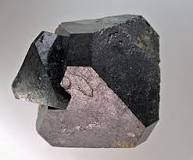
\includegraphics[scale=0.6]{peros.jpg}
\caption{Forma de la perovskita como mineral.}
\label{fig:figura1}
\end{figure}

\subsection{Abscisión de energía de fluidos mediante mini-turbinas\citep{cHolmes2015}}
Cada vez se pretenden miniaturizar mas las cosas, en el caso de la turbinas, se busca alimentar pequeños sistemas, de tamaño reducido para insértalos en rincones muy estrechos. Algunas aplica iones serian para la agricultura inteligente(donde se busca obtener energía el agua que pasa en un sistema de riego), monitoreo ambiental y hasta vigilancia y seguridad en el entorno distribuido. 

\section{Ejemplos de Energy Harvesting}
\subsection{TERM(Thermoelectric energy recovery module)}
Un TERM\citep{Kim2010} recupera el calor perdido por los transistores de amplificación de potencia. Su principal aplicación es en telecomunicaciones, sistemas inalámbricos o bien redes(internet). El calor de los semiconductores puede ser almacenados para que después sea almacenado en baterías. 

\begin{figure}[H]
\centering
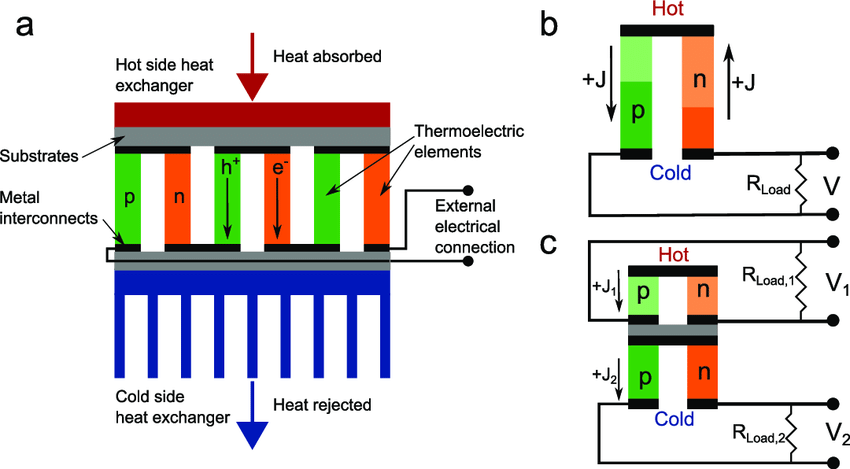
\includegraphics[scale=0.3]{term.png}
\caption{Procesos del la TERM en semiconductores.}
\label{fig:figura1}
\end{figure}
\subsection{Ventanas de vidrio transparente para la captación de energía solar}
Las ventanas de vidrio laminado transparente\citep{Alghamedi2014} para la  recolección de energía visiblemente transparentes y totalmente inorgánicas son la solución más práctica para aumentar significativamente la producción de energía fotovoltaica integrada en edificios (BIPV) al tiempo que reduce el consumo de energía relacionado con el enfriamiento y la calefacción en los edificios. Mediante la incorporación de materiales luminóforos en las capas intermedias de laminación y el uso de recubrimientos de película delgada espectralmente selectivos junto con las células solares CuInSe2, la mayor parte de la radiación solar visible puede transmitirse a través de la ventana de vidrio con una atenuación mínima, mientras que la radiación ultravioleta (UV) se convierte y en-rutados junto con una parte significativa de la radiación infrarroja a los bordes para la recolección por las células solares. Los resultados experimentales demuestran un panel de vidrio transparente de 10 cm × 10 cm que recolecta la energía de manera transparente, con una transparencia superior al 60\%, una atenuación de la energía solar invisible superior al 90\% y una potencia eléctrica cercana a los 30 Wp / m2 generada principalmente por infrarrojos (IR) y UV radiaciones. Estos resultados abren el camino para la realización de ventanas de vidrio transparente para la recolección de energía en áreas grandes y visiblemente transparentes para sistemas BIPV.

\subsection{Triboelectrificación}
La triboelectrificación\citep{Chen2018}, también conocida como electrificación por contacto, es una fenómeno común en la vida de las personas. Se ha identificado como un efecto negativo en algunas situaciones, como provocar incendios y explosión de polvo, mientras que este efecto existe en casi todas partes.Una estrategia prometedora para utilizar en lugar de reducir la triboelectrificación es convertirla y almacenarla en otras formas de energía.A pesar de la triboelectrificación\citep{Chen2018} podría ser generada por casi cualquier
material en la vida cotidiana, sigue siendo un serio desafío recopilar y convertir esta pequeña energía en potencia disponible. 

\section{Conclusión}
El campo del la recolección de energía del medio ambiente esta creciendo debido a la demanda de energía libre, que no contamine y donde se requiere que los sistemas que están actualmente sean 100\% eficiente, aprovechando la energía que se desperdicia. Las nuevas tecnologías, materiales y procesos dan el crecimiento e investigación sobre las energías "limpias", sin embargo la mayoría de estas están en desarrollo y no se tiene un producto factible. El campo del Energy Harvesting y Scavenging esta apenas comenzando.  


\bibliographystyle{unsrt}
\bibliography{ref1}

% Your document ends here!
\end{document}